\documentclass[12pt,twoside,a4paper]{article}
\usepackage{listings}
\usepackage{tcolorbox}
\usepackage{placeins}
\usepackage{hyperref}
\usepackage{float}
\newcommand{\lstfont}[1]{\color{#1}\scriptsize\ttfamily}

\lstset{
    language=[ANSI]C++,
    showstringspaces=false,
    backgroundcolor=\color{black!90},
    basicstyle=\lstfont{white},
    identifierstyle=\lstfont{white},
    keywordstyle=\lstfont{magenta!40},
    numberstyle=\lstfont{white},
    stringstyle=\lstfont{cyan},
    commentstyle=\lstfont{yellow!30},
    emph={
        cudaMalloc, cudaFree,
        __global__, __shared__, __device__, __host__,
        __syncthreads,
    },
    emphstyle={\lstfont{green!60!white}},
    breaklines=true
}


\title{GPU Computing\\
Exercise 5}
\author{
  Luis Wenzel\\
  Miro Joensuu\\
  Daniel Bayer\\
  Noah Schneider
}
\date{}

\begin{document}

\maketitle

\section{Presenting}
Willing to present:\\
5.1 Yes\\
5.2 Yes\\
5.3 Yes\\
5.4 No\\

\newpage
\section{Reading(5.1)} 
\subsection{The GPU Computing Era.}
The article describes the historical evolution of GPU computing, starting with a demand for real time graphic rendering in the late 1990s. It highlights how, with the addition of CUDA additional flexibility was added, enabling an expansion into a multitude of additional computing domain. The authors then give a quick introduction into the CUDA programming model, which shall not be explained here as it corresponds to the lecture contents. Then follows a description of several aspects of the Fermi architecture, talking about PCIe as the GPU-CPU interconnect, the memory hierarchy, streaming multiprocessors, parallel thread exectuion and the concept of CUDA cores. It concludes with a pledge for using GPU CPU coprocessing, showing how parallel intensive as well as mostly sequential programs can leverage the advantages of having both components available.\\
\newline
What can be taken away from the article is, that has been shown since, further evolution with regards to more general/generic use of GPUs might enable even more domains to leverage the advantages of GPU computing. Additionally, with the GPU CPU coprocessing, the advantages CPUs have will still remain valid, even with the further evolution of GPUs. The key takeaway is to try and make use of the availability of both components to achieve the best performance possible.\\
\newline
In general, we agree with the notion of the article to harness the power of GPU CPU coprocessing. An aspect though which is neglected in the article is the additonal space, power and monetary requirements of having a system equipped with both components. The final projection with regards to a 50\% increase in compute power per year might have been correct at the time of writing, but is very optimistic for the current state of hardware.

\newpage
\section{Matrix Multiplication}
\subsection{GPU: naive}
\begin{figure}[h]
    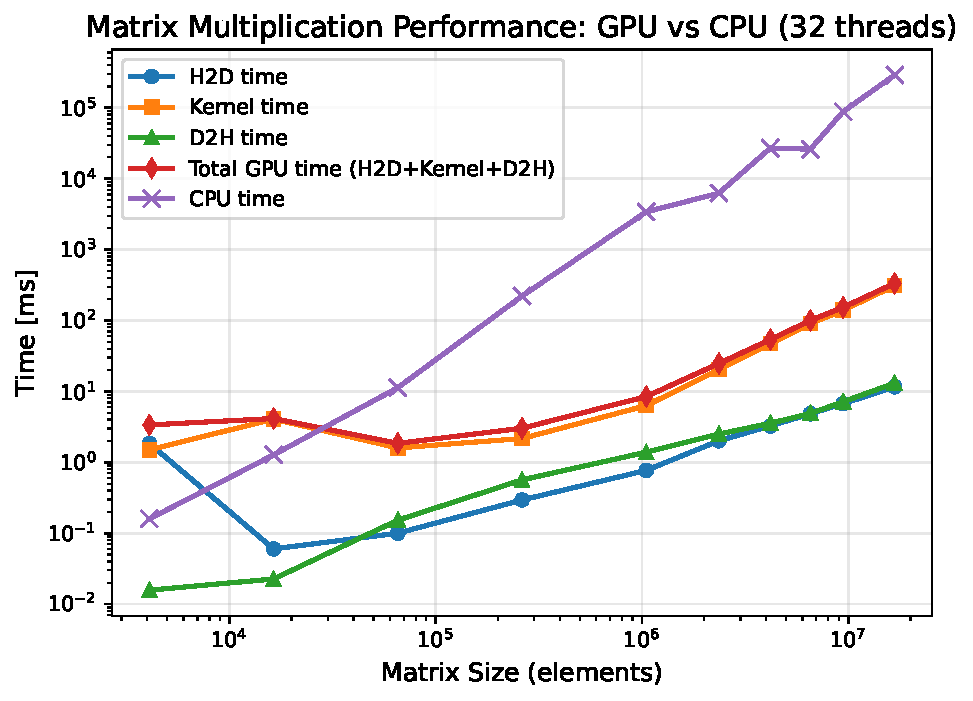
\includegraphics[scale=0.7]{../plots_miro/performance.pdf}
    \caption{Performance comparison 32 threads/block}
    \label{fig:5.2a}
\end{figure}
\ref{fig:5.2a} shows the performance of the multiplication and the data movements for different matrix sizes. While the transfer times increase with larger matrices, they are always dominated by the computation time being approx. one order of magnitude larger.\\
Compared to the version on the CPU, the comparison shows that the speedup sharply increases with matrix size until approx. 1 Million elements.\\
The maximum speedup measured is for a matrix size of 4096x4096 with a speedup of 934 for just the calculation and a speedup of 865 when including the time for the data movement.\\
\begin{figure}[h]
    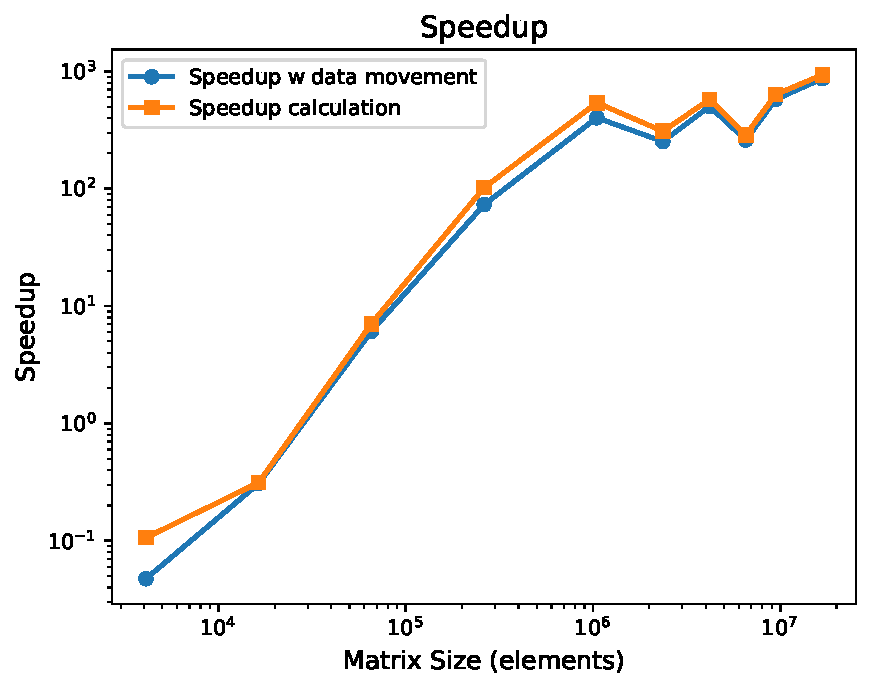
\includegraphics[scale=0.7]{../plots_miro/speedup.pdf}
    \caption{Speedup 32 threads/block}
    \label{fig:5.2b}
\end{figure}
\FloatBarrier
With regards to scaling the threads per block, we can see in \ref{fig:5.2c} and \ref{fig:5.2d} that (excluding some outliers) the runtime decreases especially for the initial increase from 1 to 8 threads per block. After that the improvements are smaller, with thread sizes which are not a power of 2 performing worse than their surrounding powers of 2.\\
\begin{figure}[h]
    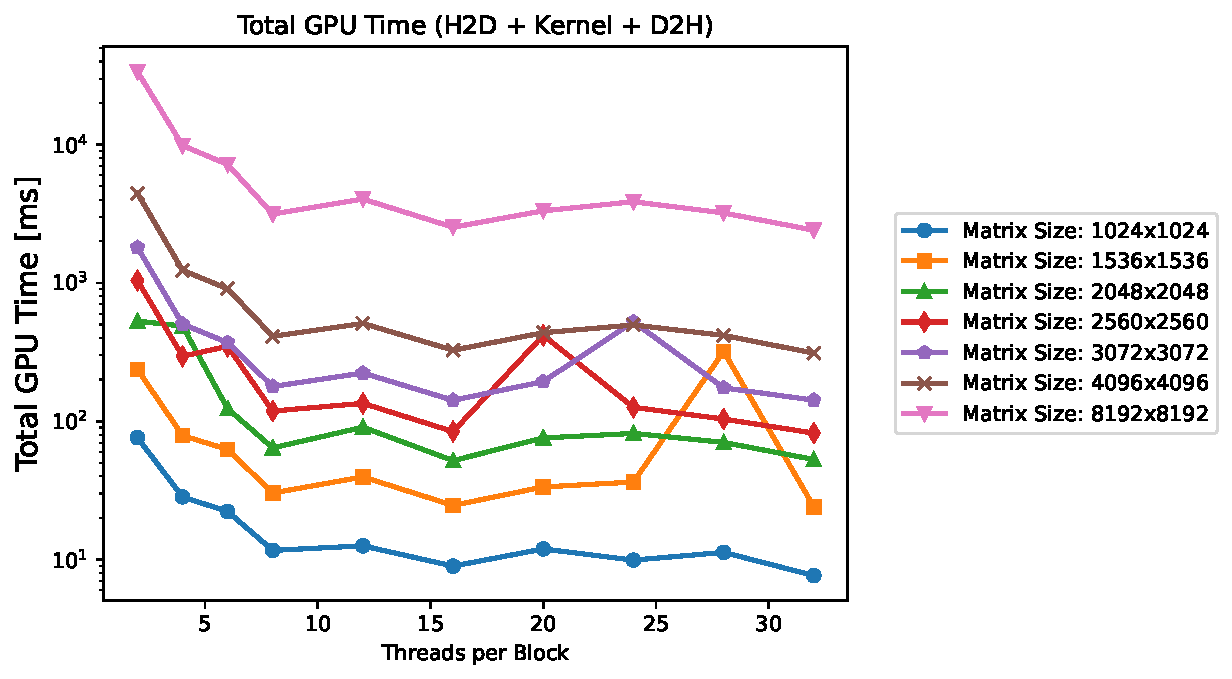
\includegraphics[scale=0.7]{../plots_miro/threads.pdf}
    \caption{Speedup 32 threads/block}
    \label{fig:5.2c}
\end{figure}
\\
\begin{figure}
    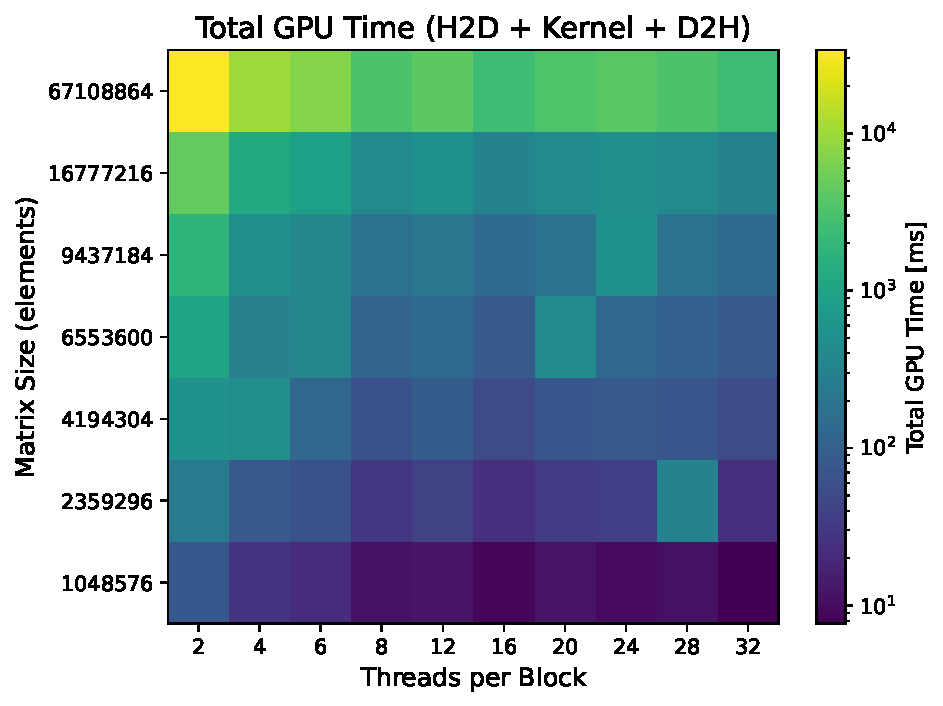
\includegraphics[scale=0.7]{../plots_miro/threads_heatmap.pdf}
    \caption{Speedup 32 threads/block}
    \label{fig:5.2d}
\end{figure}
\FloatBarrier	

\subsection{GPU: version using shared memory}
The task is split into different subtasks. For the first subtask, we measured the execution time of different threads-per-block, our chosen problem size is the size 2048 * 2048. The result shows that, with shared memory, the optimal execution time varies between the dimension of 8 on each block Size untill the range of 13 on the block size. With larger block sizes, using a problemsize of 2048*2048, the execution time worsens. This can also be seen in graphic \ref{fig:shared_vs_naive}.
\begin{figure}[h]
    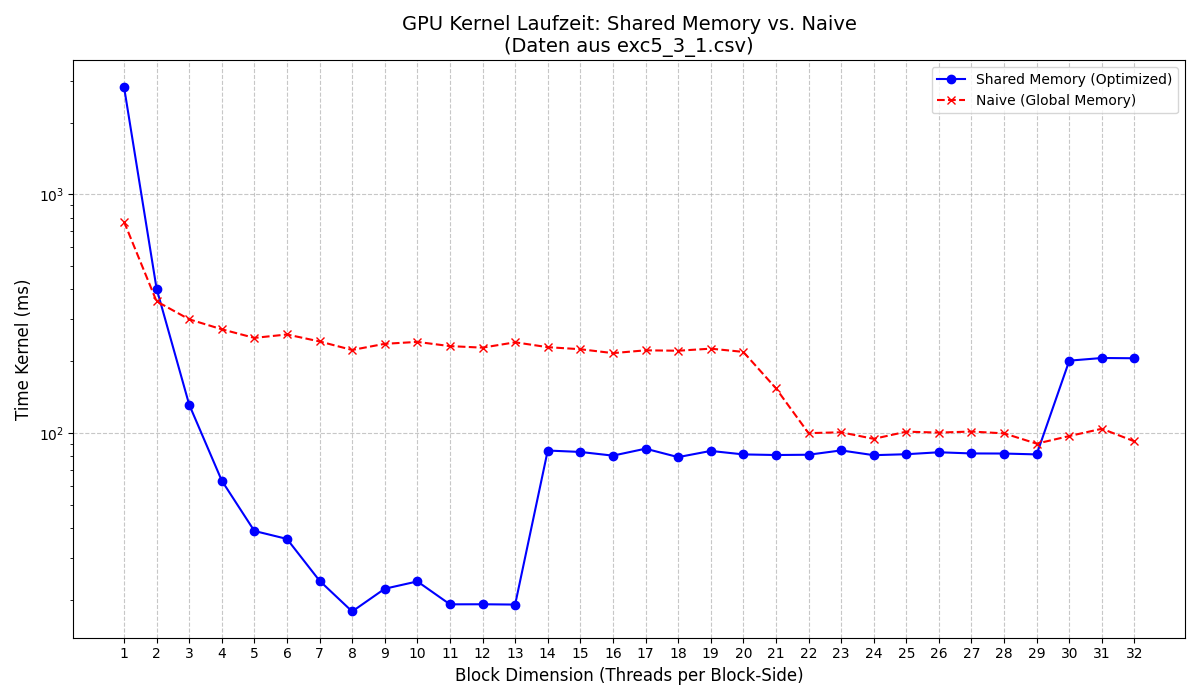
\includegraphics[width=\textwidth]{GPUKernelLaufzeitSharedMemoryVsNaive_2048_2048__LOG.png}
    \caption{Runtime in Shared Memory vs. Naive memory}
    \label{fig:shared_vs_naive}
\end{figure}
\\
The secound subtask explains the overall runtime together with different components over different problem sizes. It is visible, that with a larger problem size, the execution time increases as well. \ref{fig:shared_TOTAL} shows the steady increase in time. 
\begin{figure}[h]
    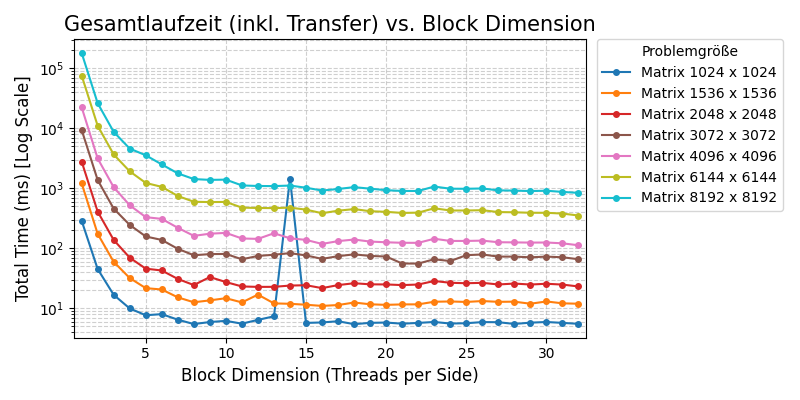
\includegraphics[width=\textwidth]{exc5_3_2_Vary_Threads_Diffrent_Problemsize.png}
    \caption{Executiontime of diffrent problemsizes by diffrent threads per Block}
    \label{fig:shared_TOTAL}
\end{figure}
The spike in the 1024 * 1024 matrix could be a loading error of the Cluster.
\\
In the last subtask of the section, the speedup from shared to naive execution is beeing explored. Hereby we explore with the Kernel Speedup the computing speedup only, and with APplicationSpeedup the overall time of the Whole programm with the H2D, D2H and Kernel time together. The chosen speedup we look at is the speeup by a blocksize of 32. A Maximum speedup faktor of 1.916 can be messured.
The results can be viewed in \ref{fig:speedup_TOTAL_2}.
\begin{figure}[h]
    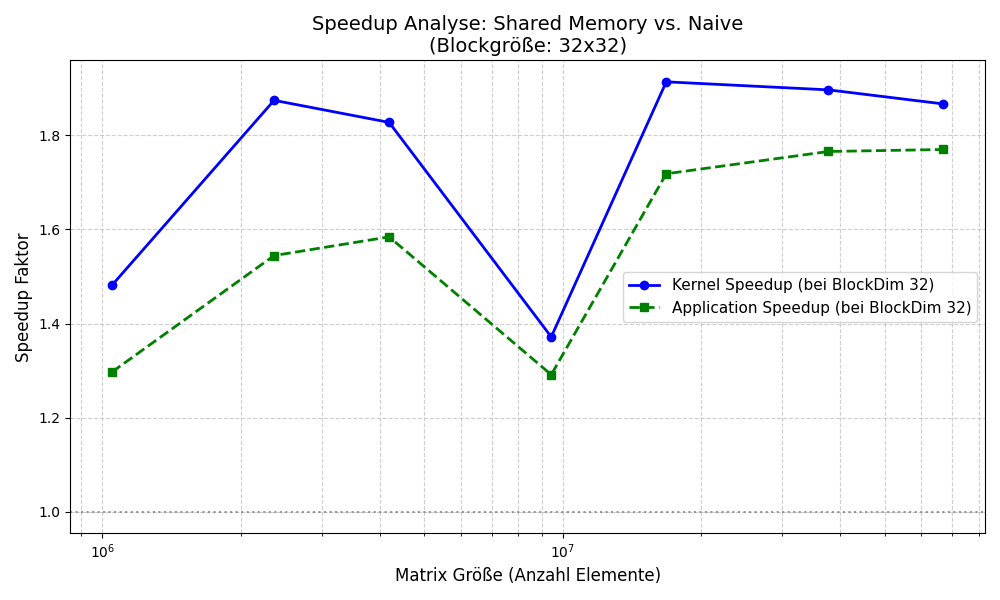
\includegraphics[width=\textwidth]{exc5_3_3_Speedup.png}
    \caption{Speedup of Kernel without and with enviroment}
    \label{fig:speedup_TOTAL_2}
\end{figure}
\FloatBarrier
\subsection{GPU: caching on}
\begin{figure}[h]
    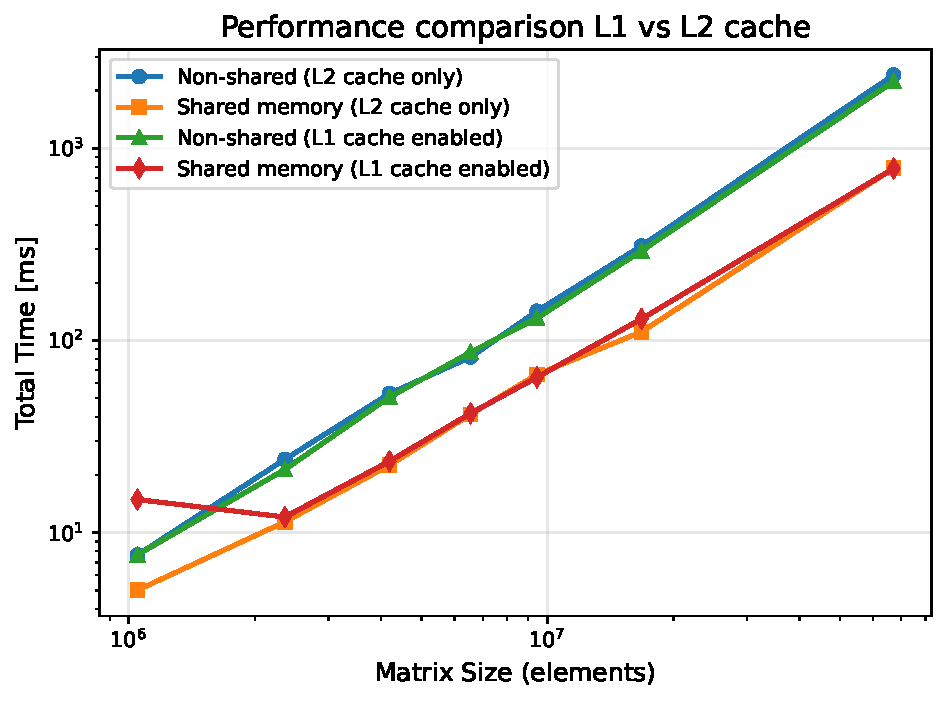
\includegraphics[width=\textwidth]{../plots_miro/performance_L1.pdf}
    \caption{L1 Cache comparison}
    \label{fig:l1}
\end{figure}

\ref{fig:l1} shows the performance comparison for a version with an enabled L1 cache. With our results, we did not identify a relevant change in performance for any of the implementations. This might be due to the choosen sizes in combination with the access patterns, or just some technical issue.
\FloatBarrier


\end{document}
